\section{Results}\label{sec:Results}
In this section we overview the results of the event selection outlined in the previous sections. Section \ref{sec:DataReduction} gives the breakdown of data events passing all our selection cuts and presents the beamline plots for this sample. Section \ref{sec:MCReduction} provides the similar breakdown of the MC events passing the selection cuts. Section \ref{sec:ValidationPlots} overviews a series of Data/MC comparisons to validate that the sample of simulated events is well reproduced in the data. Finally, Section \ref{sec:CrossSection} shows the inclusive $\pi^{-}$-Argon cross-section.


%%%%%%%%%%%%%%%%%%%%%%%%%%%%%%%%%%%%%%%%%%%%%%%%%%%
\subsection{Data Event Reduction} \label{sec:DataReduction}
%%%%%%%%%%%%%%%%%%%%%%%%%%%%%%%%%%%%%%%%%%%%%%%%%%%
Table \ref{tab:CutSummary} gives the event reduction for the negative polarity $\pi, \mu, e$ data sample for Run-I, Run-II, and combined. The definition of the cuts presented here are given in Section \ref{sec:TPCCandidateSelect}

%%% Put event reduction tables here 
\begin{table}[htb]
	\begin{center}
	\resizebox{0.95\textwidth}{!}{%
	\begin{tabular}{|c|c|c|c|}
	\hline
	%\multicolumn{5}{|c|}{\textbf{Summary of inclusive NC $\pi^{0}$ Event Selection Cuts}} \\
	%\hline \hline
	  \textbf{Event Selection} & Run-I Negative Polarity & Run-II Negative Polarity & Combined  \\
	\hline
	Total Number of Beam Events & 113,336 & 1,585,598 & 1,698,934 \\
	\hline
	$\pi, \mu, e$ Mass Selection & 20,653 & 493,455 & 514,108 \\
	\hline
	20~ns $<$TOF$<$27 & 20,577 & 485,159 & 55736 \\
	\hline
	Requiring an upstream TPC Track within $z<2$cm & 18,882  & 403,561   &  422,443 \\
	\hline
	$<4$ tracks in the first $z<14$cm & 12,910  & 316,451  & 329,361 \\
	\hline
	Electromagnetic shower rejection & 9,824  & 232,510  &  242,334 \\
	\hline
	Unique match between WC/TPC Track & 5,500 & 120,956 & 126,456\\
	\hline
	\hline
	\end{tabular}}
	\caption{Summary of the events passing the inclusive pion selection criteria.} \label{tab:CutSummary}
	\end{center}
\end{table}

For the combined Run-I/Run-II sample Figures \ref{fig:WCandTOFBeamlinePlot}, \ref{fig:DeltaXDeltaY} show the time-of-flight and momentum spectrum as well as the results of the WC/TPC matching. The addition of a cut on the TOF to require  20~ns $<$TOF$<$27 is to clean up the low momentum high TOF events seen in Figure \ref{fig:WCandTOFBeamlinePlot}.

\begin{figure}[h!]
\centering
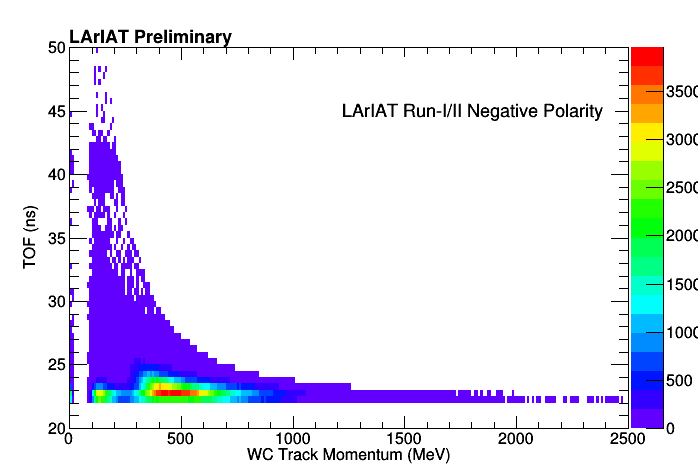
\includegraphics[scale=0.30]{./images/TOFvsWCTrk.png}
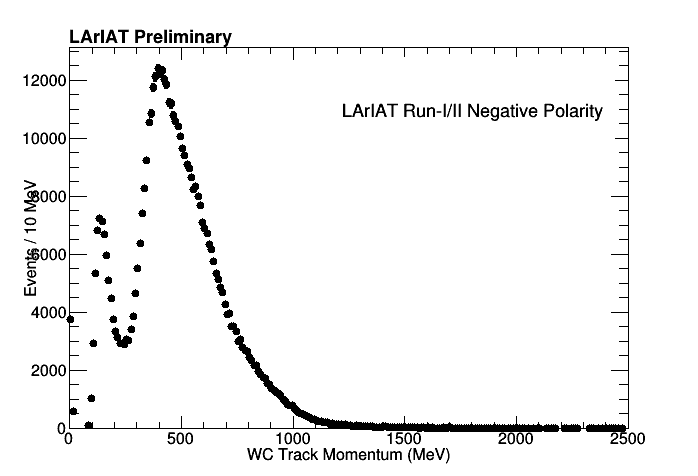
\includegraphics[scale=0.30]{./images/wctrkMomentum.png}
\caption{(Left) Time-of-Flight vs Wire Chamber Track Momentum. (Right) The momentum spectrum for our sample.}
\label{fig:WCandTOFBeamlinePlot}
\end{figure}

\begin{figure}[h!]
\centering
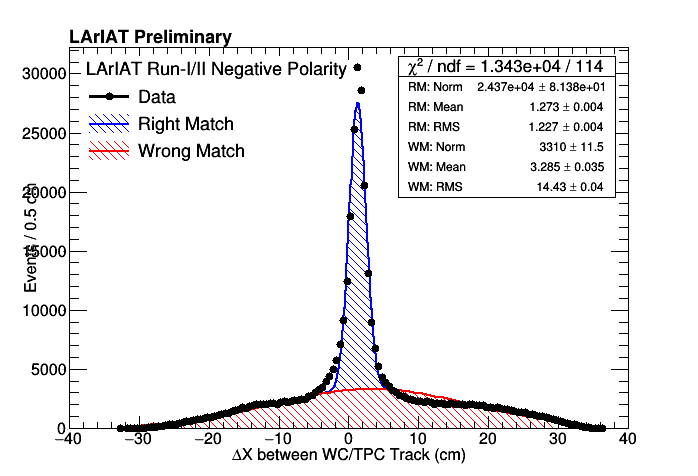
\includegraphics[scale=0.30]{./images/DeltaX.png}
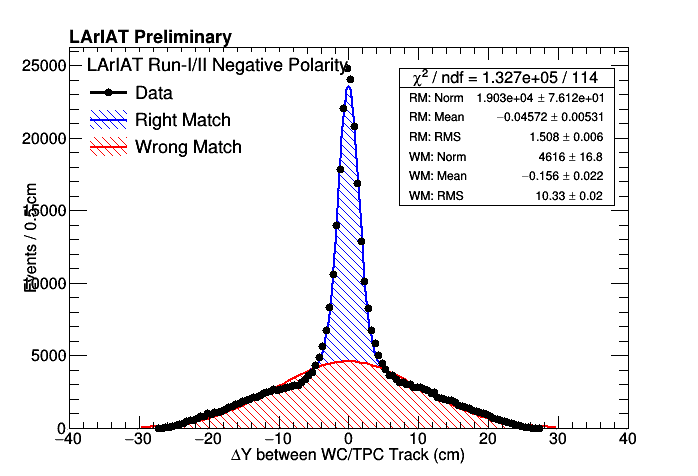
\includegraphics[scale=0.30]{./images/DeltaY.png}
\caption{The $\Delta X$ and $\Delta Y$ distributions prior to requiring the match between the TPC and WC track.}
\label{fig:DeltaXDeltaY}
\end{figure}

%%%%%%%%%%%%%%%%%%%%%%%%%%%%%%%%%%%%%%%%%%%%%%%%%%%
\subsection{MC Event Reduction} \label{sec:MCReduction}
%%%%%%%%%%%%%%%%%%%%%%%%%%%%%%%%%%%%%%%%%%%%%%%%%%%
Table \ref{tab:MCRunIICutSummary} shows a similar event reduction as was done in previous section for the sample of Run-II MC.

%%% Put event reduction tables here 
\begin{table}[htb]
	\begin{center}
	\resizebox{0.98\textwidth}{!}{%
	\begin{tabular}{|c|c|c|c|c|c|}
	\hline
	%\multicolumn{5}{|c|}{\textbf{Summary of inclusive NC $\pi^{0}$ Event Selection Cuts}} \\
	%\hline \hline
	  \textbf{Event Selection} & Run-II High Yield & Run-II High Yield & Run-II High Yield & Run-II High Yield & Run-II High Yield \\
	   & $\pi^{-}$ MC & $\mu^{-}$ MC  & $e^{-}$ MC & $K^{-}$ MC & $\gamma$ MC \\
	\hline
	Total Number of MC Events & 359,000 & 361,000 & 361,000 & 185,000 & 193,500 \\
	\hline
	MC-Particle Reaches the TPC & 245,511 & 246,874 & 323,997 & 95,391 & 72,782 \\
	\hline
	Requiring an upstream TPC Track within $z<2$cm & 220,752 & 221,966 & 254,218 & 82,407 & 5,782 \\
	\hline
	$<4$ tracks in the first $z<14$cm & 220,454 & 221,666 & 239,406 & 81,369 & 5,730 \\
	\hline
	Electromagnetic shower rejection & 218,068 & 219,274 & 94,293 & 77,281 & 2,471 \\
	\hline
	Unique match between WC/TPC Track & 180,341 & 181,327 & 46,133 & 67,420 & 1,670\\
	\hline
	\hline
	\end{tabular}}
	\caption{Summary of the MC events passing the inclusive pion selection criteria.} \label{tab:MCRunIICutSummary}
	\end{center}
\end{table}

Since the data has significantly more statistics for Run-II compared to Run-I ($\sim$22:1 ratio), the Run-II MC is used for the purposes of comparison as mixing of the two samples in this ratio does not change the final result. For the sake of completeness, Table \ref{tab:MCRunICutSummary} shows a similar event reduction as was done in previous section for the sample of Run-I MC.

%%% Put event reduction tables here 
\begin{table}[htb]
	\begin{center}
	\resizebox{0.95\textwidth}{!}{%
	\begin{tabular}{|c|c|c|c|c|c|}
	\hline
	%\multicolumn{5}{|c|}{\textbf{Summary of inclusive NC $\pi^{0}$ Event Selection Cuts}} \\
	%\hline \hline
	  \textbf{Event Selection} & Run-I High Yield & Run-I High Yield & Run-I High Yield & Run-I High Yield & Run-I High Yield \\
	   & $\pi^{-}$ MC & $\mu^{-}$ MC  & $e^{-}$ MC & $K^{-}$ MC & $\gamma$ MC \\
	\hline
	Total Number of MC Events & 357,000 &  &  & & 193,500 \\
	\hline
	MC-Particle Reaches the TPC & 258,294 &  &  & & 72,782 \\
	\hline
	Requiring an upstream TPC Track within $z<2$cm & 233,763  &  &  & & 5,782 \\
	\hline
	$<4$ tracks in the first $z<14$cm & 233,447  &  &  & & 5,730 \\ 
	\hline
	Electromagnetic shower rejection & 230,960  &  & & & 2,471 \\
	\hline
	Unique match between WC/TPC Track & 189,670 &  & & & 1,670\\
	\hline
	\hline
	\end{tabular}}
	\caption{Summary of the MC events passing the inclusive pion selection criteria.} \label{tab:MCRunICutSummary}
	\end{center}
\end{table}

Table \ref{tab:MCPercentageTable} summarizes the fraction of events passing all the inclusive pion analysis cuts. This fraction is calculated using the number of events passing all the cuts divided by the number of MC events which reach the front face of the TPC. We use the number of MC events reaching the front face of the TPC instead of the total number of MC events because using the latter would mis-represent the efficiency of the TPC based cuts.

\begin{table}[h!]
\centering
\resizebox{0.95\textwidth}{!}{%
\begin{tabular}{|c|c|c|c|c|c|}
\hline
 & $\pi^{-}$ MC & $\mu^{-}$ MC  & $e^{-}$ MC & $K^{-}$ MC & $\gamma$ MC \\
\hline
\textbf{Percent of events passing cut} & 73.5$\%$ & 73.4$\%$ & 14.2 $\%$ & 70.6$\%$ & 2.3$\%$ \\
\hline
\end{tabular}}
\caption{Fraction of MC Events passing inclusive pion analysis cuts.}
\label{tab:MCPercentageTable}
\end{table}

It should also be noted that the efficiency for selecting $K^{-}$ events is likely to be overly inflated here both because they make up a very small percentage of the negative polarity beam $< 1\%$ and because these cuts do not take into account the beamline mass filter applied to the data.


%%%%%%%%%%%%%%%%%%%%%%%%%%%%%%%%%%%%%%%%%%%%%%%%%%%
\subsection{Validation Plots} \label{sec:ValidationPlots}
%%%%%%%%%%%%%%%%%%%%%%%%%%%%%%%%%%%%%%%%%%%%%%%%%%%
In this section we will cover a few different aspects of the validation of the data and Monte Carlo samples being used here. These checks include checks of the calorimetry, validation of the reconstruction by looking at a series of low level variables in both data and MC, and cross-checks of the thin-slice method.

%%%%%%%%%%%%%%%%%%%%%%%%%%%%%%%%%%%%%%%%%%%%%%%%%%%%%%%%%%%%
\subsubsection{Calorimetry Cross-check} \label{sec:calocrosscheck}
%%%%%%%%%%%%%%%%%%%%%%%%%%%%%%%%%%%%%%%%%%%%%%%%%%%%%%%%%%%%
\paragraph{\textbf{Wire-to-Wire Corrections}}

The wire response to charge has been observed to be non-uniform during Run-I and Run-II data taking. The pattern of the wire to wire variation stays fairly consistent across various runs and has been shown to be independent from the track inclination respect to the wire planes, track distance from the wire planes (i.e. from the drift time), track position along the wire and the cold electronics. More detail about these investigations can be found in docDB-1804, with the best current hypothesis for the origin of this oscillation being the WRD cards that drove the 25' cables to the DAQ rack.


A correction factor is applied in order to restore the uniformity in the wire response to charge. The left hand side of Figure \ref{fig:wirebywire} shows the variation in the charge for each wire for a set of runs in Run-I. A mean correction factor for each wire is calculated and applied to the data to remove the effect of this non-uniform charge response. The right hand side of Figure \ref{fig:wirebywire} shows the effect of this correction on a sample of Run-I data, for the collection plane.

\begin{figure}[h!]
\centering
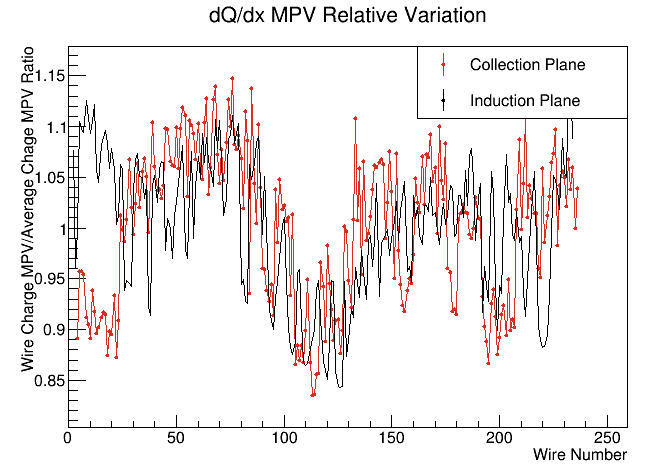
\includegraphics[scale=0.35]{./images/Run1WireCorrectionFactor.png}
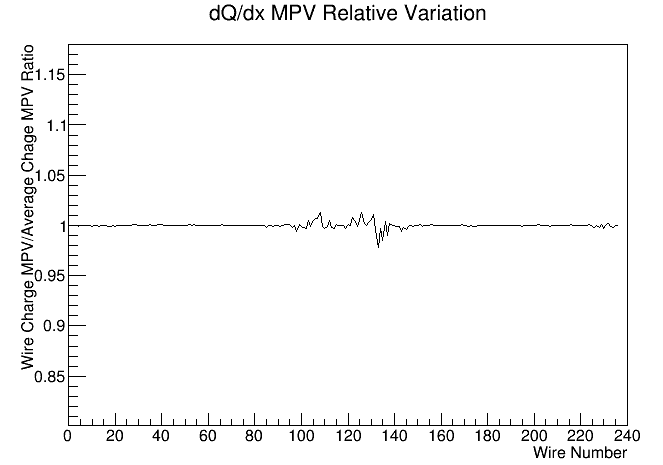
\includegraphics[scale=0.35]{./images/Run1WireCorrected.png}
\caption{(LHS): Deviation from the reference value of the $dQ/dx$ most probable value as calculated on each wire for a given plane. The reference value is obtained by averaging $dQ/dx$ over all the wires. Variations as high as 15\% are observed. Values for Induction (black) and Collection (red) planes are reported. (RHS): The corrected $dQ/dX$ response for Run-1 data sample, Collection plane only}
\label{fig:wirebywire}
\end{figure}

\paragraph{\textbf{Electron Lifetime Correction}}

The amount of charge per unit of length $dQ/dx$ collected at the wire plane is dependent on the distance traveled by the ionization charge in LAr because of quenching by the electronegative contaminants. In order to retrieve the original ionization charge, we need to correct for the attenuation factor, expressed in terms of electron lifetime and drift time. The full explanation of the method employed to measure the electron lifetime can be found in DocDb 1804.

For Run-I and Run-II data, the electron lifetime is found using a sample of cosmic rays and stored in an online database. When the samples used in this analysis are reconstructed, they have a lifetime correction applied to account for the varying lifetime seen in LArIAT. The details of how this is applied in the calorimetry package is explained in docDB-????. Figure \ref{fig:LifetimeNOchargecorrection} shows an example of the lifetime derived for Run-I and Run-II data.

\begin{figure}[h!]
\centering
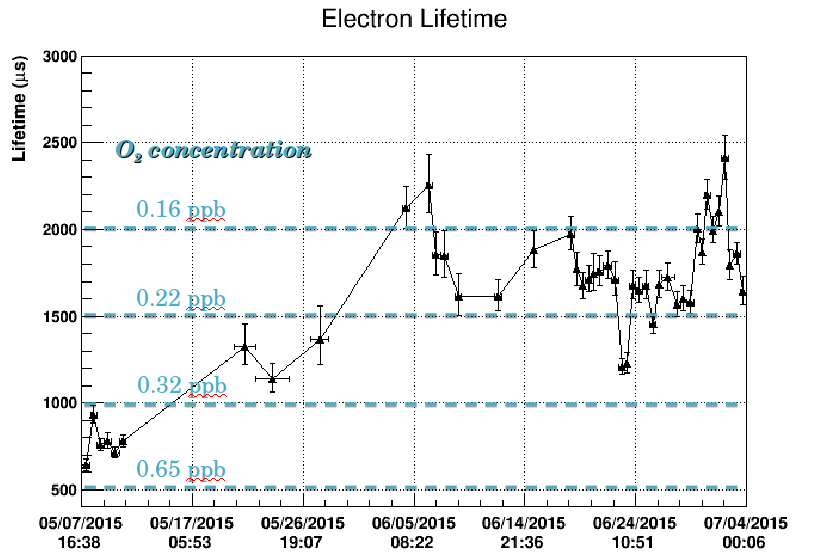
\includegraphics[scale=0.35]{./images/Run1Lifetime.png}
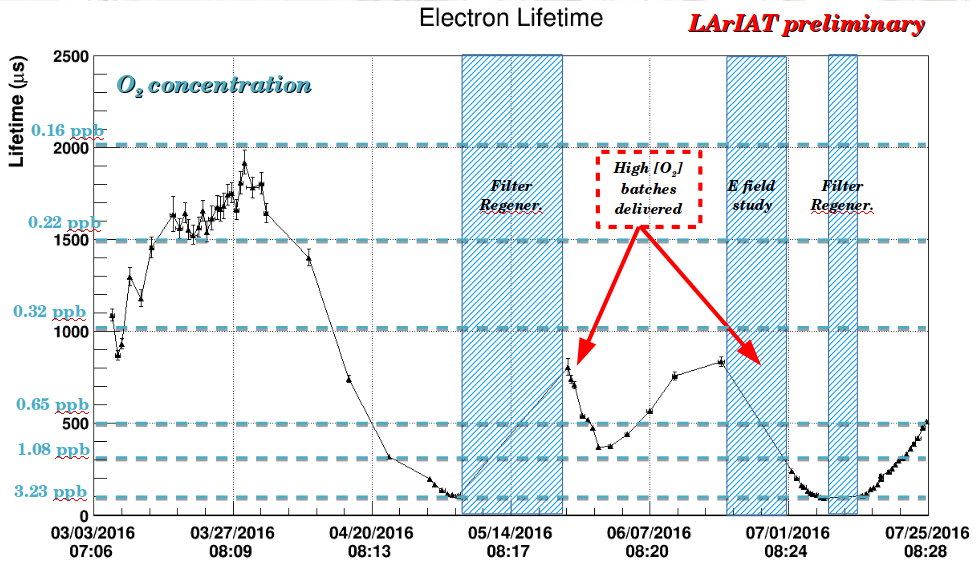
\includegraphics[scale=0.28]{./images/Run2Lifetime.png}
\caption{Electron lifetime for Run-I (Top) and Run-II (Bottom), obtained with the multi-track method (see DocDb 1804). Errors are statistical only.}
\label{fig:LifetimeNOchargecorrection}
\end{figure}

\paragraph{\textbf{Calorimetry Constant Tuning}}
The calorimetry constants used in this data analysis were determined from a sample of data and Monte Carlo spanning Run I and Run II. The calibration method, described in greater detail in docDB-????, is predicated on the Bethe-Bloch description of the mean rate of energy loss for various particle species. The basic idea of this calibration technique is to utilize a portion of a track within the LArTPC that has a well known momentum and particle species to measure the energy deposited per unit length (dE/dX) as recorded inside the TPC. Once a sample of particles dE/dX has been measured at various momentums, we then tune to calorimetry constants within the reconstruction software to align these measured values to match the theoretical ones.

Figure \ref{fig:dEdXvsMomentum} shows the calorimetry response for the $\pi, \mu, e$-High-Yield data sample used in this analysis. The selection method for this sample is to take eaccg  track within the TPC that is uniquely matched to a wire-chamber track and use the measured momentum for that track. We require the track to be of a minimum length of 10~cm long (to ensure we are away from any interaction point where the track may be broken into subsequent tracks). We then take the first twelve spacepoints of the track (excluding the first point to avoid edge effects near the field cage) and sample the reconstructed dE/dX for each point along the track. On average, this samples 5~cm of the track and takes the dE/dX measurements are then put into a histogram that corresponds to measured momentum of the track.

\begin{figure}[h!]
\centering
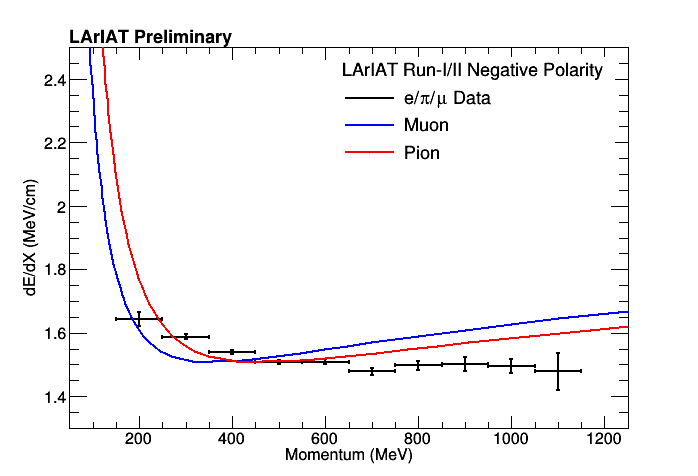
\includegraphics[scale=0.35]{./images/dEdXvsMomentumCombined.png}
\caption{dE/dX most probable value (MPV) as a function of momentum for the sample of events used in this analysis. These values are obtained using the calorimetry constants derived in docDB-????}
\label{fig:dEdXvsMomentum}
\end{figure}

\newpage
%%%%%%%%%%%%%%%%%%%%%%%%%%%%%%%%%%%%%%%%%%%%%%%%%%%%%%%%%%%%
\subsubsection{Data/MC Comparisons} \label{sec:DataMCCompare}
%%%%%%%%%%%%%%%%%%%%%%%%%%%%%%%%%%%%%%%%%%%%%%%%%%%%%%%%%%%%

Here we present a series of low-level plots which validate the data and Monte Carlo reconstruction. Each set of plots is shown with the y-axis in both linear and log scale to allow for comparisons in the bulk as well as the tale. Commentary on any set of plots is made in the caption.

\begin{figure}[h!]
\centering
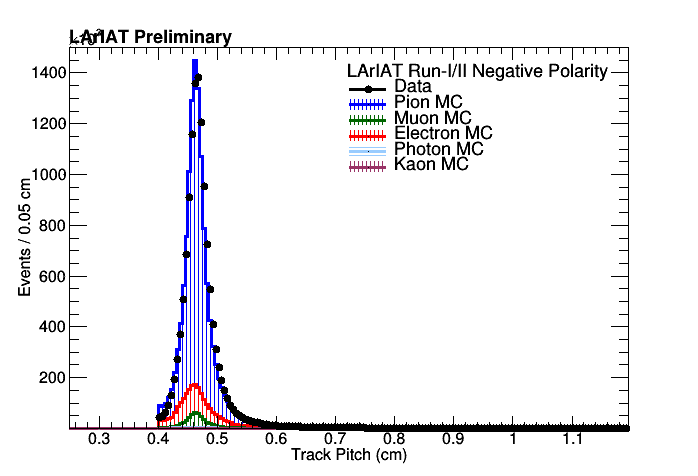
\includegraphics[scale=0.33]{./images/TrackPitch.png}
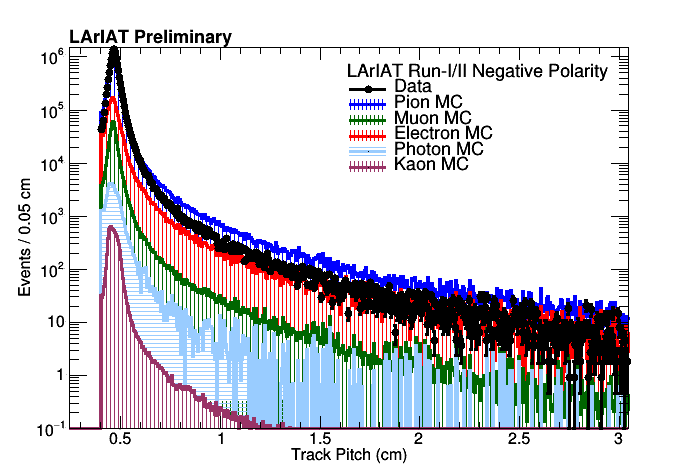
\includegraphics[scale=0.33]{./images/TrackPitchLog.png}
\caption{The reconstructed track pitch for data and Monte Carlo. Monte Carlo is scaled to data in the proportions which represent both the expected beam composition (Table \ref{tab:beamcomp1}) and the selection efficiency for that sample (Table \ref{tab:MCPercentageTable}. The data and MC agree well in the bulk of the sample, with the high end of the track pitch tail showing some disagreement, suggesting different pathologies in the data and MC cause points to be skipped along the track. These difference are quantitatively small and thus shouldn't impact the final result. }
\label{fig:DataMCTrackPitch}
\end{figure}

\begin{figure}[h!]
\centering
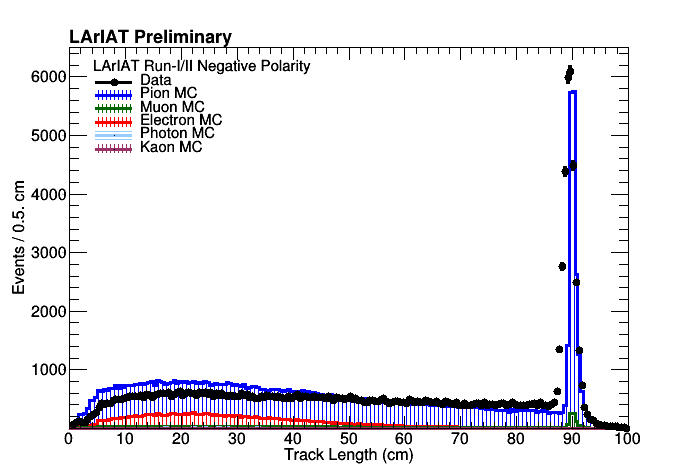
\includegraphics[scale=0.33]{./images/TrackLength.png}
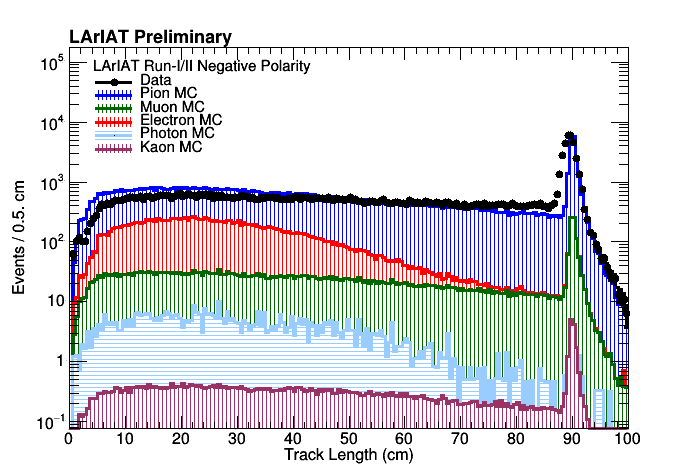
\includegraphics[scale=0.33]{./images/TrackLengthLog.png}
\caption{The reconstructed track length for data and Monte Carlo. Monte Carlo is scaled to data in the proportions which represent both the expected beam composition (Table \ref{tab:beamcomp1}) and the selection efficiency for that sample (Table \ref{tab:MCPercentageTable}. The data and MC agree overall with the MC slightly over-predicting the shortest tracks where the electron and photon samples dominate. Later plots show these slight difference to be negligible to the overall analysis.}
\label{fig:DataMCTrackLength}
\end{figure}

\begin{figure}[h!]
\centering
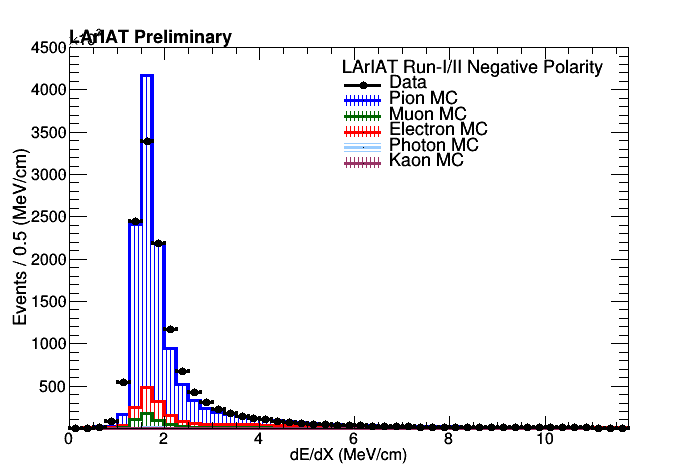
\includegraphics[scale=0.33]{./images/dEdX.png}
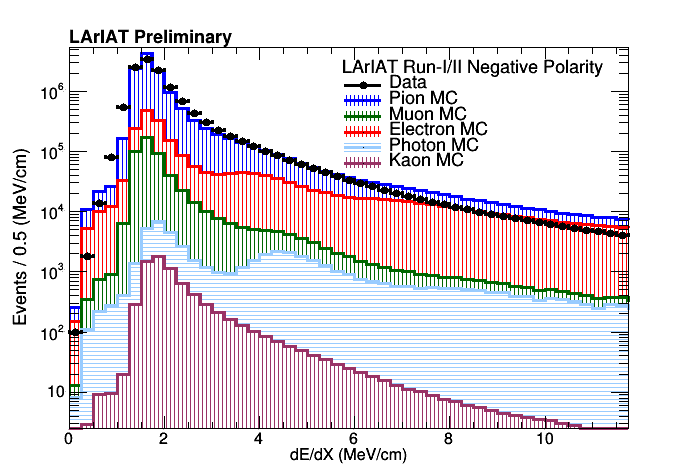
\includegraphics[scale=0.33]{./images/dEdXLog.png}
\caption{The reconstructed energy deposited per unit length (dE/dX) for data and Monte Carlo. Monte Carlo is scaled to data in the proportions which represent both the expected beam composition (Table \ref{tab:beamcomp1}) and the selection efficiency for that sample (Table \ref{tab:MCPercentageTable}. The data and MC agree in the most probable value (MPV) and in the shape. There is a slight difference in the highest side tail for the dE/dX $>$ 6 MeV/cm. This corresponds to a very small overall component of the sample and thus should only cause a slight difference in the computation of the kinetic energy for the track.}
\label{fig:DataMCdEdX}
\end{figure}

\begin{figure}[h!]
\centering
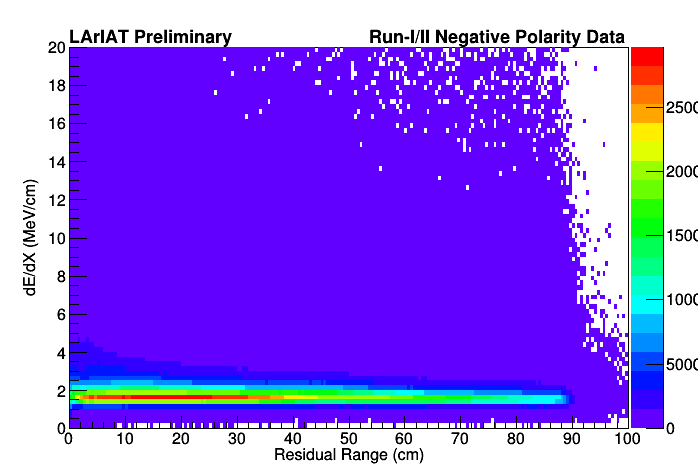
\includegraphics[scale=0.33]{./images/dEdXvsRRData.png}
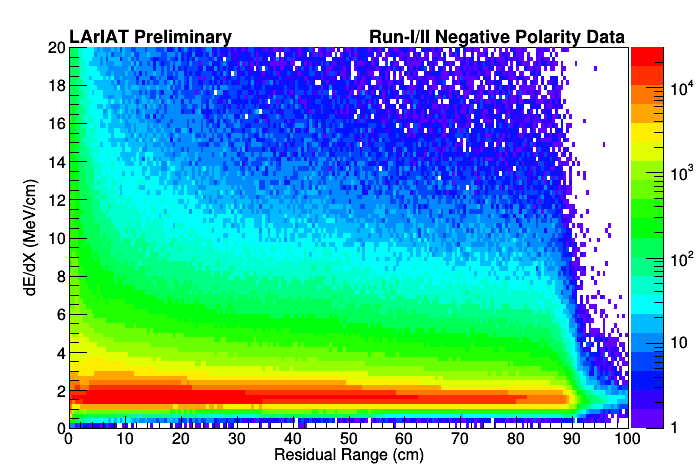
\includegraphics[scale=0.33]{./images/dEdXvsRRDataLog.png}
\caption{The reconstructed energy deposited per unit length (dE/dX) versus the Residual  Range for the data sample selected in Table \ref{tab:CutSummary}. These results agree well with Figure \ref{fig:PionMCdEdXvsRR} giving confidence that the sample of data is dominated by minimum ionizing particles (such as pions) and that the samples are well calibrated.}
\label{fig:DatadEdXvsRR}
\end{figure}

\begin{figure}[h!]
\centering
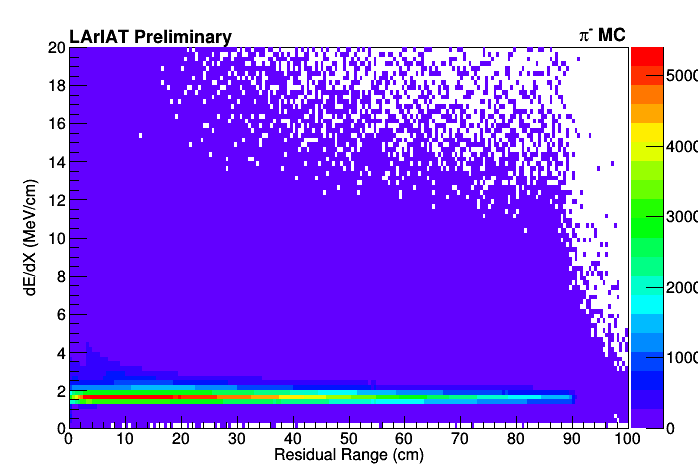
\includegraphics[scale=0.33]{./images/dEdXvsRRPionMC.png}
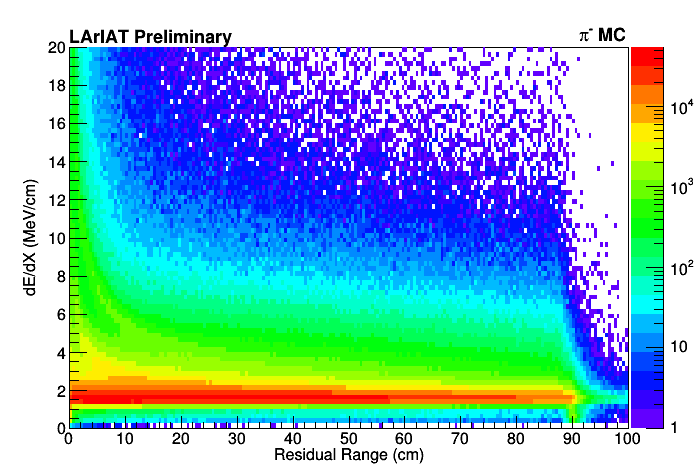
\includegraphics[scale=0.33]{./images/dEdXvsRRPionMCLog.png}
\caption{The reconstructed energy deposited per unit length (dE/dX) versus the Residual  Range for the Pion MC sample selected in Table \ref{tab:MCRunIICutSummary}.}
\label{fig:PionMCdEdXvsRR}
\end{figure}


\newpage
%%%%%%%%%%%%%%%%%%%%%%%%%%%%%%%%%%%%%%%%%%%%%%%%%%%
\subsection{Inclusive $\pi^{-}$-Argon Cross-Section} \label{sec:CrossSection}
%%%%%%%%%%%%%%%%%%%%%%%%%%%%%%%%%%%%%%%%%%%%%%%%%%%